\documentclass[12pt,]{krantz}
\usepackage{lmodern}
\usepackage{setspace}
\setstretch{2}
\usepackage{amssymb,amsmath}
\usepackage{ifxetex,ifluatex}
\usepackage{fixltx2e} % provides \textsubscript
\ifnum 0\ifxetex 1\fi\ifluatex 1\fi=0 % if pdftex
  \usepackage[T1]{fontenc}
  \usepackage[utf8]{inputenc}
\else % if luatex or xelatex
  \ifxetex
    \usepackage{xltxtra,xunicode}
  \else
    \usepackage{fontspec}
  \fi
  \defaultfontfeatures{Ligatures=TeX,Scale=MatchLowercase}
\fi
% use upquote if available, for straight quotes in verbatim environments
\IfFileExists{upquote.sty}{\usepackage{upquote}}{}
% use microtype if available
\IfFileExists{microtype.sty}{%
\usepackage{microtype}
\UseMicrotypeSet[protrusion]{basicmath} % disable protrusion for tt fonts
}{}
\usepackage[a4paper,tmargin=2.5cm,bmargin=2.5cm,lmargin=3.5cm,rmargin=2.5cm]{geometry}
\usepackage[unicode=true]{hyperref}
\PassOptionsToPackage{usenames,dvipsnames}{color} % color is loaded by hyperref
\hypersetup{
            pdftitle={Bookdown中文书稿写作手册},
            pdfauthor={汤银才},
            colorlinks=true,
            linkcolor=Maroon,
            citecolor=Blue,
            urlcolor=Blue,
            breaklinks=true}
\urlstyle{same}  % don't use monospace font for urls
\usepackage[style=gb7714-2015ay,refsegment=chapter,gblocal=chinese,gbnamefmt=lowercase,gbnamefmt=familyahead,gbtype=false,maxbibnames=99]{biblatex}
\addbibresource{book.bib}
\addbibresource{packages.bib}
\usepackage{color}
\usepackage{fancyvrb}
\newcommand{\VerbBar}{|}
\newcommand{\VERB}{\Verb[commandchars=\\\{\}]}
\DefineVerbatimEnvironment{Highlighting}{Verbatim}{commandchars=\\\{\}}
% Add ',fontsize=\small' for more characters per line
\usepackage{framed}
\definecolor{shadecolor}{RGB}{248,248,248}
\newenvironment{Shaded}{\begin{snugshade}}{\end{snugshade}}
\newcommand{\AlertTok}[1]{\textcolor[rgb]{0.94,0.16,0.16}{#1}}
\newcommand{\AnnotationTok}[1]{\textcolor[rgb]{0.56,0.35,0.01}{\textbf{\textit{#1}}}}
\newcommand{\AttributeTok}[1]{\textcolor[rgb]{0.77,0.63,0.00}{#1}}
\newcommand{\BaseNTok}[1]{\textcolor[rgb]{0.00,0.00,0.81}{#1}}
\newcommand{\BuiltInTok}[1]{#1}
\newcommand{\CharTok}[1]{\textcolor[rgb]{0.31,0.60,0.02}{#1}}
\newcommand{\CommentTok}[1]{\textcolor[rgb]{0.56,0.35,0.01}{\textit{#1}}}
\newcommand{\CommentVarTok}[1]{\textcolor[rgb]{0.56,0.35,0.01}{\textbf{\textit{#1}}}}
\newcommand{\ConstantTok}[1]{\textcolor[rgb]{0.00,0.00,0.00}{#1}}
\newcommand{\ControlFlowTok}[1]{\textcolor[rgb]{0.13,0.29,0.53}{\textbf{#1}}}
\newcommand{\DataTypeTok}[1]{\textcolor[rgb]{0.13,0.29,0.53}{#1}}
\newcommand{\DecValTok}[1]{\textcolor[rgb]{0.00,0.00,0.81}{#1}}
\newcommand{\DocumentationTok}[1]{\textcolor[rgb]{0.56,0.35,0.01}{\textbf{\textit{#1}}}}
\newcommand{\ErrorTok}[1]{\textcolor[rgb]{0.64,0.00,0.00}{\textbf{#1}}}
\newcommand{\ExtensionTok}[1]{#1}
\newcommand{\FloatTok}[1]{\textcolor[rgb]{0.00,0.00,0.81}{#1}}
\newcommand{\FunctionTok}[1]{\textcolor[rgb]{0.00,0.00,0.00}{#1}}
\newcommand{\ImportTok}[1]{#1}
\newcommand{\InformationTok}[1]{\textcolor[rgb]{0.56,0.35,0.01}{\textbf{\textit{#1}}}}
\newcommand{\KeywordTok}[1]{\textcolor[rgb]{0.13,0.29,0.53}{\textbf{#1}}}
\newcommand{\NormalTok}[1]{#1}
\newcommand{\OperatorTok}[1]{\textcolor[rgb]{0.81,0.36,0.00}{\textbf{#1}}}
\newcommand{\OtherTok}[1]{\textcolor[rgb]{0.56,0.35,0.01}{#1}}
\newcommand{\PreprocessorTok}[1]{\textcolor[rgb]{0.56,0.35,0.01}{\textit{#1}}}
\newcommand{\RegionMarkerTok}[1]{#1}
\newcommand{\SpecialCharTok}[1]{\textcolor[rgb]{0.00,0.00,0.00}{#1}}
\newcommand{\SpecialStringTok}[1]{\textcolor[rgb]{0.31,0.60,0.02}{#1}}
\newcommand{\StringTok}[1]{\textcolor[rgb]{0.31,0.60,0.02}{#1}}
\newcommand{\VariableTok}[1]{\textcolor[rgb]{0.00,0.00,0.00}{#1}}
\newcommand{\VerbatimStringTok}[1]{\textcolor[rgb]{0.31,0.60,0.02}{#1}}
\newcommand{\WarningTok}[1]{\textcolor[rgb]{0.56,0.35,0.01}{\textbf{\textit{#1}}}}
\usepackage{longtable,booktabs}
% Fix footnotes in tables (requires footnote package)
\IfFileExists{footnote.sty}{\usepackage{footnote}\makesavenoteenv{long table}}{}
\usepackage{graphicx,grffile}
\makeatletter
\def\maxwidth{\ifdim\Gin@nat@width>\linewidth\linewidth\else\Gin@nat@width\fi}
\def\maxheight{\ifdim\Gin@nat@height>\textheight\textheight\else\Gin@nat@height\fi}
\makeatother
% Scale images if necessary, so that they will not overflow the page
% margins by default, and it is still possible to overwrite the defaults
% using explicit options in \includegraphics[width, height, ...]{}
\setkeys{Gin}{width=\maxwidth,height=\maxheight,keepaspectratio}
\setlength{\emergencystretch}{3em}  % prevent overfull lines
\providecommand{\tightlist}{%
  \setlength{\itemsep}{0pt}\setlength{\parskip}{0pt}}
\setcounter{secnumdepth}{5}
% Redefines (sub)paragraphs to behave more like sections
\ifx\paragraph\undefined\else
\let\oldparagraph\paragraph
\renewcommand{\paragraph}[1]{\oldparagraph{#1}\mbox{}}
\fi
\ifx\subparagraph\undefined\else
\let\oldsubparagraph\subparagraph
\renewcommand{\subparagraph}[1]{\oldsubparagraph{#1}\mbox{}}
\fi

% set default figure placement to htbp
\makeatletter
\def\fps@figure{htbp}
\makeatother


\usepackage{ctex}
\usepackage{ctexheading}

\usepackage{bm}
\usepackage{mathrsfs}

%%%%% Theorems
\usepackage[amsmath,thref,thmmarks,hyperref]{ntheorem}
\theorempostskipamount0em
\theoremstyle{plain}
\theoremheaderfont{\normalfont\heiti\color{black}}
\theorembodyfont{\normalfont\kaishu\color{black}}
\theoremindent0em
\theoremseparator{\hspace{0.2em}}
\theoremnumbering{arabic}
\newtheorem{theorem}{定理}[chapter]
\newtheorem{lemma}[theorem]{引理}
\newtheorem{corollary}[theorem]{推论}
\newtheorem{proposition}[theorem]{命题}
\newtheorem{property}[theorem]{性质}
\newtheorem{definition}{定义}[chapter]
\newtheorem{remark}{注记}[chapter]
\newtheorem{assumption}{假设}[chapter]



%
%\theoremheaderfont{\normalfont\itshape\color{blue}}
\theorembodyfont{\normalfont\rmfamily\color{black}}
\newtheorem{example}{例}[chapter]

\theoremstyle{nonumberplain}
\theorempreskip{0em}
\theoremsymbol{\ensuremath{\Box}}
\newtheorem{proof}{证明}


\usepackage{makeidx}
    


\makeindex



\title{Bookdown中文书稿写作手册}
\author{汤银才}
\date{2021-07-21}

\begin{document}
\maketitle


\thispagestyle{empty}

\allowdisplaybreaks
]%   而\allowdisplaybreaks[4]则是强制换页等同于\allowdisplaybreaks
%---------------------------- 数学公式设置 ------------------------------%
\setlength{\abovedisplayskip}{8pt plus1pt minus1pt}     %公式前的距离
\setlength{\belowdisplayskip}{8pt plus1pt minus1pt}     %公式后面的距离
\setlength{\arraycolsep}{2pt}   %在一个array中列之间的空白长度, 因为原来的太宽了


\frontmatter

{
\setcounter{tocdepth}{2}
\tableofcontents
}
\listoftables
\listoffigures
\hypertarget{ux524dux8a00}{%
\chapter*{前言}\label{ux524dux8a00}}


\indent

今年接了5本与贝叶斯近似计算包\texttt{INLA}相关的翻译书,将由高等教育出版社出版。在准备翻译的时候,我静下来思考了一下二个问题。一是互联网时代在兼顾图书质量的同时怎么充分考虑读者阅读体验?二是什么是当下最为成熟的图书写作工具?特别是与数据科学密切相关的统计类图书的写作与出版。书稿模板的选择成为首先要考虑的事。

在书稿模板的选择与测试过程中遇到了很多的坑,幸运的是逐个踩过来了,但从\(\TeX\)到\texttt{Rnw} (Sweave+R), 再到\texttt{Rmd} (Knitr + R), 最后到\texttt{Bookdown}, 共经历了4个模板。快速、高效、高质量是写书人追求的目标。目前来看\texttt{Bookdown}是最好的选择,因为它满足我模板选择的快速编辑、高效生成、高质量输出的要求。

这本小册子可视为一个写中文书稿的\texttt{Bokdown}模板,也是中文\texttt{Bookdown}写作的一本说明书,其中汇总了书稿中几大核心要素的写作技巧。我主要参考了三个模板\texttt{Bookdown}模板和三本电子书,罗列如下,在此一并对谢益辉、李东风等表示感谢。

\begin{enumerate}
\def\labelenumi{\arabic{enumi}.}
\item
  谢益辉, \href{https://github.com/yihui/bookdown-chinese}{bookdown 中文范例}
\item
  谢益辉, \href{https://github.com/yihui/bookdown-crc}{A bookdown example for Chapman \& Hall books}
\item
  \href{https://github.com/rstub/bookdown-chapterbib}{bookdown-chapterbib}
\item
  谢益辉, bookdown: \href{https://bookdown.org/yihui/bookdown/}{Authoring Books and Technical Documents with R Markdown}, 2021-03-15.
\item
  李东风,R语言教程,\href{https://www.math.pku.edu.cn/teachers/lidf/docs/Rbook/html/_Rbook/bookdown.html}{第23章:用bookdown制作图书}, 2020-12-28.
\item
  Yihui Xie, J. J. Allaire, Garrett Grolemund, \href{https://bookdown.org/yihui/rmarkdown/}{R Markdown: The Definitive Guide}, 2020-12-14.
\end{enumerate}

\mainmatter

\hypertarget{intro}{%
\chapter{引言}\label{intro}}

\indent

这是第\ref{intro}章的内容,回顾中国图书发展的历史及最新趋势. \autocite{xie2015,R-base},

\hypertarget{sec1-1}{%
\section{中国图书出版的变化}\label{sec1-1}}

\indent

中国的图书出版经历一些折腾,方正系统一度非常流行,但现在看来是非常失败的,主要是它在解决公式排版的同时没有解决便利性,其本质上想实现在其自创的中文系统中将\(\TeX\)命令做一个映射以实现数学公式排版,同时完成格式的定制。

中国学术界也经历了一些折腾,如中科院张林波研究员等开发的\texttt{CCT}系统和华东师范大学肖刚与陈志杰等老师开发的天元系统,它们是\(\TeX\)系统汉化版,较好地解决了汉字生成与调用,但因没有考虑普适性或可拓展性而像方正系统一样随着\texttt{CJK}的逐渐成熟而逐渐被抛弃,均退出了历史舞台。而同期中科院吴凌云博士等在普及\(\TeX\)的同时开发的\(\TeX\)中文套餐\(C\TeX\)相当成功,主要是针对汉字排版的\texttt{ctex}宏包,并对三个主流的文档类\texttt{book}, \texttt{article}, \texttt{report}进行了定制,推出了相应的中文文档类\texttt{ctexbook}, \texttt{ctexart}, \texttt{ctexrep}, 由此避免了传统的基于\texttt{CJK}宏包需要的大幅定制,同时保证了与原有\(\TeX\)系统的兼容性。这样我们始终可以使用跨平台的\texttt{TeXLiVe}进行排版或各类模板的开发,例如各个出版社的图书模板、各个期刊的模板、各高校的硕士和博士毕业论文模板等。

\(\TeX\)的出现\footnote{是伟大的\texttt{Knuth}创造了排版的奇迹},而且始终屹立不倒的原因是什么? 第一个原因是它解决了一个\texttt{Word}之类文字编辑系统的痛点,即从所见所得(WYSIWYG, What you see is what you get)到所想所得(WYTIWYG), 即通过一些\(\TeX\)命令集构成一个完整的编程语言,由它完成一个封闭的体系,具有类似\texttt{C}语言一样非常强大的开发功能,由此形成了后来的\texttt{latex}, \texttt{miktex}, \texttt{latex2.09}, \texttt{luatex}, \texttt{xetex}等\(\TeX\)编译引擎,它们在充分利用电脑系统资源的同时实现高质量输出需要的精度。

\(\TeX\)屹立不倒的另一个原因是浮动对象的处理,即包括公式,表格、图形、页码、章节、文献、定理等的标签化与引用,实现文档内部的自由跳转,结合\texttt{Acrobat\ Reader}这样强大的\texttt{pdf}阅读器的支持,使得读者的阅读体验得到大幅改善,并为图书的电子化奠定了基础。

随着数据科学这一新兴学科的出现,开源的\texttt{R}和\texttt{Python} (还有正在逐步流行的\texttt{Julia})编程语言越来越强大。 为了增加这类图书的可读性,需要将代码较完整地呈现在读者面前,并且要求代码的即时可复现能力,即数据的变化,其分析的结果(包括图形和表格)也随之发生变化。这就是现在逐步流行的文学化编程(\texttt{literate\ programming}), 它实现上最早也是\(\TeX\)的鼻祖Knuth提出的, 后来被谢益辉得到重视并广泛推广,并通过\texttt{Rstudio}传递给\texttt{R}的用户。我们姑且把这种将写作与数据分析相结合的统计分析称为文学化统计编程(\texttt{literate\ statistical\ programming}), 在为数据科学爱好者带来便利的同时也通过\texttt{Bookdown}为图书的写作和电子化带来了极大的好处,越来越多的网页版电子书出现在(\url{https://bookdown.org/)和(https://github.com/)等网站上}。

现在写书选择什么类型的模板,下面我们来作进一步的探索与比较。

\hypertarget{sec1-2}{%
\section{统计类图书的核心要素}\label{sec1-2}}

\indent

统计类图书的排版除普通图书的页面及文字风格等静态元素外,核心要素体现在浮动的对象上,使得图书的阅读体验更好地发挥出来,即在不同页面之间快速切换、跟踪、搜索,必要的\texttt{R}和\texttt{Python}代码以语法高亮方式显示。

\begin{enumerate}
\def\labelenumi{\arabic{enumi}.}
\item
  \textbf{章节标题}是浮动的,最主要用于书签的生成;
\item
  \textbf{公式}是浮动的,这是数学、统计等理科书的特点,公式引用必不可少;
\item
  \textbf{图形}是浮动的,统计图形作为可视工具,在说明数据或展示分析结果时经常会引用相应的图形;
\item
  \textbf{表格}是浮动的,通常是原始数据或统计分析的结果以表格形式展示出来,它们可能被多次在不同的章节中引用;
\item
  \textbf{定理}是浮动的, 这里定理是指与之相关的一大类,包括常用的定理、引理、推论、命题、例子等,它们在文中也会被反复引用;
\item
  \textbf{文本}可以设置浮动标签后被引用,最为常见的是图形与表格的题图(caption)通过文本方式来引用;
\item
  \textbf{文献}是浮动的,这在是谈及前人的已有工作、成果比较或进行综述时经常要引用大量已经发表的论文、图书、会议报告等.
\end{enumerate}

\(\TeX\)有一套成熟的浮动对象的排版方式,通过给浮动对象打标签(label),然后引用(ref), \texttt{Bookdown}思路一样,但比\(\TeX\)的处理稍复杂些(可能因不习惯引起)。我们在后面章节中分别举例说明。

\hypertarget{sec1-3}{%
\section{统计数据分析类图书模板的选择}\label{sec1-3}}

\indent

统计数据分析类图书既有理论或原理的讲解,又会有一些案例分析,包括这些案例分析实现的代码。我们可以考虑的模板主要有三种类型。

\hypertarget{sec1-3-1}{%
\subsection{\texorpdfstring{基于纯 \(\TeX\) 模板}{基于纯 \textbackslash TeX 模板}}\label{sec1-3-1}}

\indent

全世界90\%的书是由\(\TeX\)排版的,包括硕士和博士毕业论文模板,这要感谢鼻祖Knuth!开源成就了\(\TeX\)!

如果仅仅是统计理论方面的书集,这显然是最好的选择,因为高质量公式的排版离不开\(\TeX\). 基于\(\TeX\)的排版存在三个明显的缺陷或不足:

\begin{enumerate}
\def\labelenumi{\arabic{enumi}.}
\item
  大量的\(\TeX\)命令需要记忆;
\item
  对于代码的排版非常不便,特别是\texttt{R}或\texttt{Python}代码执行后的输出,尤其是图形与表格;
\item
  代码以\texttt{listing}等包来呈现, 无法实时呈现代码运行的结果,不符合文学化编程的要求.
\end{enumerate}

\hypertarget{sec1-3-2}{%
\subsection{\texorpdfstring{\texttt{R}markdown与\(\TeX\)的结合}{Rmarkdown与\textbackslash TeX的结合}}\label{sec1-3-2}}

\indent

数据科学时代更注重文学化统计编程,\textbf{代码伴随}是这类图书的特点,自Springer出版\texttt{R}系列统计图书后,这种风格成为新趋势,大大方便了数据科学爱好者``便学习便练习''的学习方式。

针对代码伴随,早期对这类图书有二个解决方案:

\begin{enumerate}
\def\labelenumi{\arabic{enumi}.}
\tightlist
\item
  Sweave/knitr + \texttt{R}
\end{enumerate}

本质上它是在 \(\TeX\) 嵌入\texttt{R}代码块,并由\texttt{R}在后台运行后将结果也嵌入到\(\TeX\)中,再由\(\TeX\)的编译引擎生成\texttt{pdf}。这个方案的基本沿用\(\TeX\)的方式,它仅解决了上面提到的第二个问题。在数据科学时代,报告的快速生成成为新的要求,效率优先!随着\texttt{knitr}的出现\texttt{Sweave}退出舞台.

\begin{enumerate}
\def\labelenumi{\arabic{enumi}.}
\setcounter{enumi}{1}
\tightlist
\item
  \texttt{Rmarkdown} + \texttt{Mathjax}/\(\TeX\)
\end{enumerate}

\texttt{Markdown}作为一种轻量级的标记语言成为网页作为文字主要载体的互联网时代首先的写作工作,但它显然不适合数学与统计类论文或图书的撰写,但\texttt{knitr}和\texttt{pandoc}的出现使不同风格的内容整合与转换成为可能,而不同风格的内容各有善长的工具实现,作为统计类专业论文或图书类文档主要的内容有:

\begin{enumerate}
\def\labelenumi{\alph{enumi}.}
\item
  文字, 由markdown完成
\item
  公式,由\(\TeX\)完成
\item
  代码,由\texttt{R} (或Python) 完成
\end{enumerate}

要说明的是,在网页端,\(\TeX\)的实现可由\texttt{Mathjax}来完或渲染(转化或生成标准的公式),见第\ref{formulas}章说明。

随着\texttt{Rstudio}的越来越成熟与强大(得益于许多优秀包的出现,如\texttt{knitr}, \texttt{kableExtra}), \texttt{Rstudio}不仅是一个很好的代码编辑器(\texttt{Eidtor}), 也是一个非常好的集成开发环境(\texttt{IDE}),同时正在成为一个非常优秀的论文、幻灯片及图书等撰写与出版系统(\texttt{PUB})。后者的基本流程是

\begin{enumerate}
\def\labelenumi{\arabic{enumi}.}
\item
  由\texttt{rmd}文件通过\texttt{knitr}完成初步集成
\item
  由\texttt{pandoc}完成由\texttt{rmd}向\texttt{md}的转化与融合
\item
  由\texttt{pandoc}完成由\texttt{md}转化为\(\TeX\), 并由\texttt{laTeX}编译生成\texttt{pdf} (形式多样!)
\item
  或由\texttt{pandoc}由\texttt{md}转化为\texttt{html}, 其中的数学公式由\texttt{Mathjax}完成渲染.
\end{enumerate}

\hypertarget{sec1-3-3}{%
\subsection{\texorpdfstring{\texttt{Rmarkdown}向\texttt{Bookdown}过渡}{Rmarkdown向Bookdown过渡}}\label{sec1-3-3}}

\indent

在科技高度发达的互联系时代,读者使用的媒介基本有三类:较为专业的电脑,较为轻便的平板(电脑)和全功能的智能手机。前者以\texttt{pdf}类图书为主呈现给读者,同时可以完成标注等工作;后者以文字型的电子图书为主,消磨时间为主;而平板的使用者逐渐成为电子类图书的新势力,包括\texttt{pdf}和\texttt{epub}之类的电子书。
\texttt{Bookdown}注重不同类型读者的媒体使用的差异,并很好地实现统一编写与差异化输出。目前\texttt{Bookdown}可以生成三类图书:

\begin{enumerate}
\def\labelenumi{\arabic{enumi}.}
\item
  \texttt{gitbook},可自由出版在\texttt{git\ pages}上
\item
  \texttt{epub}, 发表到大量的电子图书平台上
\item
  \texttt{pdf}, 正规的图书出版公司以电子或纸质形式出版
\end{enumerate}

\printbibliography[segment=\therefsegment, heading=subbibliography, title={参考文献}]

\hypertarget{bookdown}{%
\chapter{\texorpdfstring{\texttt{bookdown}速览}{bookdown速览}}\label{bookdown}}

\indent

这是第\ref{bookdown}章的内容,概要性地讲解基于\texttt{bookdown}拓展包进行图书排版的整体思路与实现方式. \autocite{xie2015,R-base}

\hypertarget{sec2-1}{%
\section{\texorpdfstring{关于\texttt{bookdown}}{关于bookdown}}\label{sec2-1}}

\indent

\texttt{bookdown}扩展包(\url{https://github.com/rstudio/bookdown}) 是继\texttt{knitr}和\texttt{rmarkdown}扩展包之后, 另一个增强\texttt{markdown}格式的扩展, 使得\texttt{Rmd}格式可以支持公式、定理、图表、文献自动编号和引用等适用于编写书籍的功能。 在\texttt{bookdown}的管理下一本书的内容可以按章节分解成多个\texttt{Rmd}文件, 其中可以包含可执行的\texttt{R}代码, \texttt{R}代码生成的统计汇总结果、表格、图形可以自动插入到生成的内容中, 表格和图形可以是浮动排版的。书的输出格式包括支持\texttt{gitbook}格式的网页图书, 也可以经\(\LaTeX\)编译器转换的\texttt{PDF}图书,还 可以生成\texttt{ePub}等格式的电子书。建议使用\texttt{RStudio}集成环境来编辑、管理和生成这样的图书,可通过其内建的一键式编译整本书的插件(\texttt{build})实现。

\hypertarget{sec2-2}{%
\section{快速排版的思路}\label{sec2-2}}

\begin{enumerate}
\def\labelenumi{\arabic{enumi}.}
\item
  由\texttt{rmarkdown}完成整个书稿的写作;
\item
  由\texttt{\_output.yml}完成不同形式呈现的书稿的设计,其中\texttt{bookdown::gitbook}负责\texttt{html}形式的\texttt{gitbook}, \texttt{bookdown::pdf\_book} 负责\texttt{pdf}形式的电子书(由\(\TeX\)支持);\texttt{bookdown::epub\_book}负责\texttt{epub}电子书. 部分针对书稿简单设置可放在\texttt{index.Rmd}文件的\texttt{yml}头部(具体放在前面两组三个短线\texttt{-\/-\/-}之间);
\item
  书稿按章节进行拆分,借助\texttt{js}支持的\texttt{html}快速生成书稿的初稿,最后再进行整合,根据需要通过\texttt{Build}插件完成\texttt{gitbook}, \texttt{pdf\_book}, \texttt{epub}的构建;
\item
  借助\texttt{mathjax}处理数学公式的渲染;

  尽快可通过联网由\texttt{cdn}上的\texttt{mathjax.js}进行渲染,但速度随因公式的增加,渲染变得很慢,甚至出错。\texttt{mathjax}的本地化是提速的主要解决方案. 详见第\ref{mjx}章介绍;
\item
  重点做好章节、数学公式、表格、图形、定理、文献等浮动对象的处理,在编写过程中及时做好标签设定与引用,见\ref{sec2-6}节的汇总表格及后续各章的介绍与示例.
\end{enumerate}

\hypertarget{sec2-3}{%
\section{书的基本设置}\label{sec2-3}}

\indent

一本用\texttt{bookdown}管理的书, 一般放置在某个子目录下,并作为一个\texttt{RStudio}项目(project)用\texttt{RStudio}管理。该目录中的所有的文本文件都要使用\texttt{UTF-8}编码。

\hypertarget{index.rmdux6587ux4ef6}{%
\subsection{\texorpdfstring{\texttt{index.Rmd}文件}{index.Rmd文件}}\label{index.rmdux6587ux4ef6}}

\indent

一本\texttt{bookdown}书, 一般都需要有一个\texttt{index.Rmd}文件, 这是最后生成的网站的主页的原始文件. 这个文件的开始是\texttt{YAML}元数据部分, 进行全书的有关设置,包括标题、作者、日期及影响全书的一些选项等,放在三个减号组成的两行之间。然后写一些这本书的说明,如书的前言部分。\texttt{index.Rmd}中\texttt{YAML}元数据部分的一个例子如下:

\begin{verbatim}
title: "bookdown书稿模板"
author: "汤银才"
date: "2021-07-21"
documentclass: book
bibliography: [myrefs.bib]
biblio-style: apa
link-citations: yes
site: bookdown::bookdown_site
description: "bookdown写书体验非常好."
\end{verbatim}

注意:

\begin{enumerate}
\def\labelenumi{\arabic{enumi}.}
\item
  \texttt{site}选项很重要, 一定要有, \texttt{site:\ bookdown::bookdown\_site}使得\texttt{RStudio}能辨认这是一个\texttt{bookdown}图书项目, 从而为其生成一键编译的\texttt{build}快捷方式;
\item
  在\texttt{bookdown}项目中与\texttt{index.Rmd}同级的所有\texttt{.Rmd}文件都自动作为书的一章,其好处是作者可以任意地增删章节,编译整本书时将按照文件名的字典序依次进行。实际上, 也可以在\texttt{\_output.yml}文件中设置一项\texttt{rmd\_files}, 列出所有需要作为一章的文件,并以列出次序编译;
\item
  在\texttt{index.Rmd}的元数据中也可以指定一些\(\LaTeX\)的选项, 例如
\end{enumerate}

\begin{verbatim}
fontsize: 12pt
indent: true
linestretch: 2.0
link-citations: yes
colorlinks: yes
lot: true
lof: true
geometry:
- a4paper
- tmargin=2.5cm
- bmargin=2.5cm
- lmargin=3.5cm
- rmargin=2.5cm
\end{verbatim}

\hypertarget{bookdown.ymlux6587ux4ef6}{%
\subsection{\texorpdfstring{\texttt{\_bookdown.yml}文件}{\_bookdown.yml文件}}\label{bookdown.ymlux6587ux4ef6}}

\indent

一个\texttt{bookdown}图书项目除了\texttt{index.Rmd}文件之外,还有一些设置文件从\texttt{index.Rmd}文件的元数据部分抽离出来。 一个是\texttt{\_bookdown.yml}文件, 它存放与整本书的处理有关的\texttt{YAML}元数据。 例如

\begin{verbatim}
book_filename: "bookdown-template"
new_session: yes
language:
  label:
    fig: "图 "
    tab: "表 "
    thm: '定理'
    def: '定义'
    exm: '例'
    proof: '证明: '
  ui:
    chapter_name: ["第 ", " 章"]
\end{verbatim}

其中\texttt{new\_session:\ true}设置很重要,这使得每一个\texttt{Rmd}文件中的\texttt{R}程序都在一个单独的\texttt{R}会话中独立地运行,避免了不同\texttt{Rmd}文件之间同名变量和同名标签的互相干扰。 \texttt{book\_filename}是最终生成的\texttt{PDF}图书或者\texttt{ePub}电子书的主文件名。 \texttt{language}下可以定制一些与章节名、定理名等有关的名称。

\hypertarget{output.ymlux6587ux4ef6}{%
\subsection{\texorpdfstring{\texttt{\_output.yml}文件}{\_output.yml文件}}\label{output.ymlux6587ux4ef6}}

\indent

另一个设置文件是\texttt{\_output.yml}, 用于图书输出格式的设置\footnote{这部分内容也可以包含在\texttt{index.Rmd}的元数据部分}, 本小删子的\texttt{\_output.yml}文件内容如下

\begin{verbatim}
bookdown::gitbook:
  css: css/style.css
  split_by: chapter
  includes:
    in_header: _header.html
  config:
    toc:
      collapse: subsection
      scroll_highlight: yes
      before: |
        <li><a href="./">bookdown排版模板</a></li>
      after: |
        <li><a href="https://bookdown.org" target="blank">本书由 bookdown 强力驱动</a></li>
    download: [pdf, epub]
    edit: https://github.com/yihui/bookdown-chinese/edit/master/%s
    sharing:
      github: yes
      facebook: no
  pandoc_args: [ "--csl", "apa-6th-edition-no-ampersand.csl" ]
bookdown::pdf_book:
  includes:
    in_header: latex/preamble.tex
    before_body: latex/before_body.tex
    after_body: latex/after_body.tex
  keep_tex: yes
  dev: "cairo_pdf"
  latex_engine: xelatex
  citation_package: biblatex
  template: latex/template.tex
  toc_depth: 3
  toc_unnumbered: no
  toc_appendix: yes
  quote_footer: ["\\begin{flushright}", "\\end{flushright}"]
  pandoc_args: [ "--top-level-division=chapter" ]
bookdown::epub_book:
  stylesheet: css/style.css
  pandoc_args: [ "--csl", "apa-6th-edition-no-ampersand.csl" ]
\end{verbatim}

它分别对\texttt{gitbook}、\texttt{pdf\_book}和\texttt{epub\_book}三种输出格式设置了一些输出选项。其中一些选项是通过文件形式给出设置的,我们再补充说明一下。

\begin{enumerate}
\def\labelenumi{\arabic{enumi}.}
\item
  \texttt{style.css}是自定义的CSS显示格式,在\texttt{gitbook}和\texttt{epub\_book}中使用;
\item
  \texttt{\_header.html}是插入了一部分个性化的\texttt{HTML}代码,其内容将出现在每个生成的\texttt{HTML}文件的\texttt{head}部分。我们在此文件中给出了使用本地的\texttt{Mathjax}实现数学公式离线显示的设置,内容为
\end{enumerate}

\begin{verbatim}
<script type="text/x-mathjax-config">
MathJax.Hub.Config({
  jax: ["input/TeX","output/SVG"],
  extensions: ["tex2jax.js","MathMenu.js","MathZoom.js"],
  TeX: {
    Macros: {
      bm: ["{\\boldsymbol #1}",1],
    }, 
    extensions: ["AMSmath.js","AMSsymbols.js","noErrors.js","noUndefined.js"]
  }
});

</script>
<script type="text/javascript"
  src="http://127.0.0.1/MathJax/MathJax.js">
</script>
\end{verbatim}

其中\texttt{http://127.0.0.1/MathJax/}是本地服务器上\texttt{Mathjax}的位置。有关\texttt{Mathjax}的本地安装与启动可参考第\ref{mjx}章的介绍;

\begin{enumerate}
\def\labelenumi{\arabic{enumi}.}
\setcounter{enumi}{2}
\item
  \texttt{apa-6th-edition-no-ampersand.csl} 是\texttt{gitbook}和\texttt{epub\_book}处理文献使用的风格文件;
\item
  \texttt{preamble.tex}是处理(编译)\texttt{bookdown}文件经\texttt{pandoc}转化生成的\texttt{tex}文件时导言区需要额外的宏包和设置;
\item
  \texttt{before\_body.tex} 是\texttt{tex}书稿类正文前面的设置,最基本的是
\end{enumerate}

\begin{verbatim}
 \frontmatter
\end{verbatim}

\begin{enumerate}
\def\labelenumi{\arabic{enumi}.}
\setcounter{enumi}{5}
\tightlist
\item
  \texttt{after\_body.tex} 是\texttt{tex}书稿类正文之后的设置,最基本的是
\end{enumerate}

\begin{verbatim}
\backmatter
\end{verbatim}

\begin{verbatim}
7. `template.tex` 是针对`bookdown`编译经`pandoc`转化生成的`tex`文件时的模板,由它生成供`latex_engine`指定的编译方式(`xelatex`)编译的`tex`文件. `index.Rmd`及`_output.yml`中的设置会嵌入到这个模板中,生成完整的单文档`tex`源文件.   
\end{verbatim}

其他选项说明:

\begin{enumerate}
\def\labelenumi{\arabic{enumi}.}
\item
  \texttt{split\_by:\ chapter}: 按章分割书稿;
\item
  \texttt{collapse:\ subsection}: 目录中隐藏子节(仅显示二级标题);
\item
  \texttt{scroll\_highlight:\ yes}: 目录滚动时高亮显示,便于定位;
\item
  \texttt{keep\_tex:\ yes}: 保留中间生成的\texttt{tex}源文件,便于查错;
\item
  \texttt{dev:\ "cairo\_pdf"}: 使用\texttt{cairo\_pdf()}生成 \(\LaTeX\) 编译需要的图片文件;
\item
  \texttt{latex\_engine:\ xelatex}: \texttt{TeX}文件的排版引擎为\(Xe\LaTeX\), 针对\texttt{UTF-8}编码;
\item
  \texttt{citation\_package:\ biblatex}: 文献引用库指定为\texttt{biblatex}, 另一个为\texttt{natbib};
\item
  \texttt{toc\_depth:\ 3}: 目录提取至三级标题;
\item
  \texttt{toc\_unnumbered:\ no}: 指定目录编号;
\item
  \texttt{toc\_appendix:\ yes}: 附录添加到目录中.
\end{enumerate}

\hypertarget{sec2-4}{%
\section{章节结构}\label{sec2-4}}

\indent

如前所述, 除了\texttt{index.Rmd}文件, 项目中每个\texttt{.Rmd}文件都作为一章,其第一行是以一个\texttt{\#}号和空格开头的一级标题。

每一章可以有若干节与子节,分别用\texttt{markdown}的二级标题(二个\texttt{\#}开始)和三级标题(三个\texttt{\#}开始)编写。\texttt{bookdown}的章、节、子节标题单独成一行,其后可以添加标签, 章节的标签是标题后加空格,然后是大括号内以\texttt{\#}号开头的标签, 如

\begin{verbatim}
# 引言 {#intro}

## 关于bookdown {#bookdown}
\end{verbatim}

\texttt{bookdown}中有二个特殊的标题:

\begin{enumerate}
\def\labelenumi{\arabic{enumi}.}
\item
  部分

  内容相近的章节可以作为一个``部分''。 为此,在一个部分的第一个章节文件的章标题前面增加一行, 以\texttt{\#\ (PART)} 开头, 以\texttt{\{-\}}结尾,例如
\end{enumerate}

\begin{verbatim}
   # (PART) bookdown中的浮动对象 {-}
\end{verbatim}

\begin{enumerate}
\def\labelenumi{\arabic{enumi}.}
\setcounter{enumi}{1}
\item
  附录

  一本书的最后可以有附录, 附录的章节将显示为\texttt{A.1}, \texttt{B.1}这样的格式。 为此, 在附录章节的第一个文件开头加如下的第一行标题行:
\end{enumerate}

\begin{verbatim}
   # (APPENDIX) 附录 {-}

   # biblatex介绍 {#biber}
\end{verbatim}

\hypertarget{sec2-5}{%
\section{书的编译}\label{sec2-5}}



\indent

在\texttt{index.Rmd}或者\texttt{\_bookdown.yml}中设置\texttt{site:\ bookdown::bookdown\_site}后, \texttt{RStudio}就能识别这个项目是一个\texttt{bookdown}项目, 这时\texttt{RStudio}会有一个\texttt{Build}按钮,其中有\texttt{Build\ book}快捷图标, 从下拉菜单中选择一个输出格式(包括\texttt{gitbook}、\texttt{pdf\_book}、\texttt{epub\_book}), 就可以编译整本书(见图\ref{fig:fig2-1})。

\begin{figure}
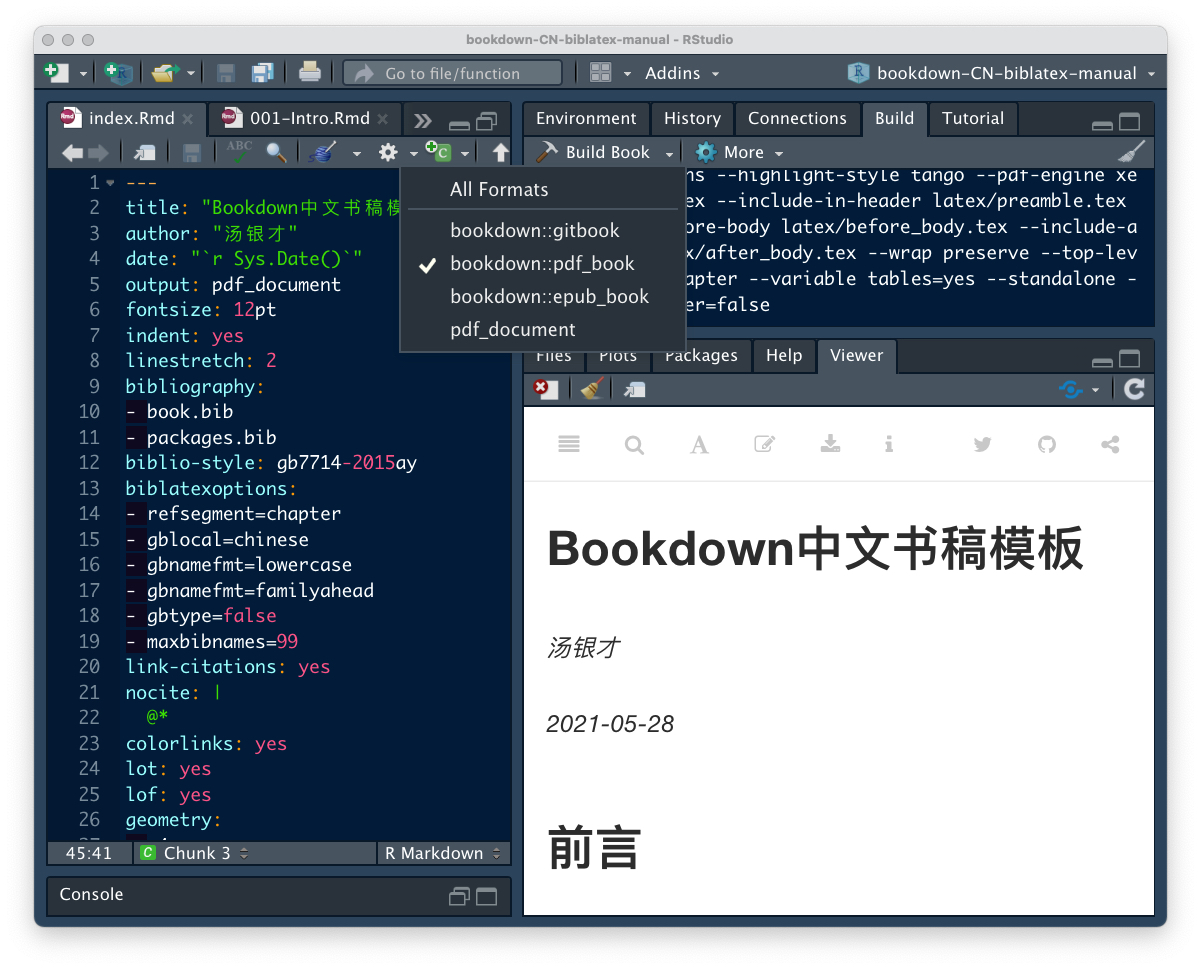
\includegraphics[width=0.85\linewidth]{./figures/Rbookdown-compile} \caption{R Bookdown编译界面.}\label{fig:fig2-1}
\end{figure}

经\texttt{build}编译生成的图书默认保存在\texttt{\_book}子目录中\footnote{可以在\texttt{\_bookdown.yml}中设置\texttt{output\_dir}项改变图书保存的子目录.}。

\begin{enumerate}
\def\labelenumi{\arabic{enumi}.}
\item
  对\texttt{gitbook}格式(即\texttt{HTML}网页格式), 编译完成后会弹出一个预览窗口, 点击``Show in new window''按钮可以将内容在操作系统默认的网络浏览器中打开。我们也可以用其他浏览器(建议使用Google chrome浏览器)打开\texttt{\_book}子目录中的\texttt{index.html}文件来查看\texttt{gitbook}格式的图书。
\item
  对于\texttt{pdf\_book}格式,如果成功编译\footnote{需要\(\LaTeX\)支持,建议安排\texttt{TeXLive},也可以仅安装谢益辉为\texttt{rmarkdown}开发的\texttt{tinytex}}, 也会弹出一个\texttt{PDF}预览窗口。 可以在\texttt{\_book}子目录中找到这个\texttt{PDF}文件。
\item
  对于\texttt{epub\_book}格式,如果成功编译,会在操作系统默认的\texttt{ePub}软件(如苹果电脑的\texttt{book})中打开,并在\texttt{\_book}子目录中找到这个\texttt{ePub}文件。
\end{enumerate}

\hypertarget{sec2-6}{%
\section{浮动对象标签与引用汇总}\label{sec2-6}}

\begin{longtable}[]{@{}rll@{}}
\toprule
浮动对象 & 标签设置 & 引用格式 \\
\midrule
\endhead
标题 & \texttt{(\#\ label)} & \texttt{\textbackslash{}@ref(label)} \\
公式 & \texttt{(\textbackslash{}\#eq:label)} & \texttt{\textbackslash{}@ref(eq:label)} \\
图形 & \texttt{label="label"} & \texttt{\textbackslash{}@ref(fig:label)} \\
表格 & \texttt{label="label"} & \texttt{\textbackslash{}@ref(tab:label)} \\
定理 & \texttt{label="label"} & \texttt{\textbackslash{}@ref(prefix:label)} \\
文本 & \texttt{(ref:label)} & \texttt{\textasciigrave{}(ref:label)\textasciigrave{}} \\
文献 & \texttt{biblabel} & \texttt{@biblabel} \\
\bottomrule
\end{longtable}

注:

\begin{enumerate}
\def\labelenumi{\arabic{enumi}.}
\item
  定理泛指定理类,包括定理(thm)、引理(lem)、推论(cor)、命题(prp)、设想(cnj)、定义(def)、例子(exm)、习题(exr)等, 其中括号中是引用时的前缀(prefix);
\item
  文本标签在单独一行中设定,可用在表格与图形的\texttt{caption}中引用,即在 \texttt{fig.caption}, \texttt{tab.caption}选项的设置中引用;
\item
  定理类环境标签前缀的汉化可在\texttt{\_bookdown.yml}中通过\texttt{language}进行\footnote{图形与表格也可同理汉化},例如
\end{enumerate}

\begin{verbatim}
language:
  label:
    fig: "图 "
    tab: "表 "
    thm: '定理'
    def: '定义'
    exm: '例'
\end{verbatim}

\printbibliography[segment=\therefsegment, heading=subbibliography, title={参考文献}]

\hypertarget{sections}{%
\chapter{Bookdow中 的章节标题}\label{sections}}

\indent

我们在第\ref{sections}章讲述章节标题的设置、标签与引用. \autocite{xie2015,bookdown2016}

\hypertarget{sec3-1}{%
\section{章节标题}\label{sec3-1}}

\indent

章节标题用遵从\texttt{markdown}的规则,用\texttt{\#}设置,

\begin{itemize}
\item
  一级标题用一个 \texttt{\#}, 在bookdown中表示\texttt{章}, 相当于\(\TeX\)中的\texttt{\textbackslash{}chapter\{\}}
\item
  二级标题用二个 \texttt{\#}, 在bookdown中表示\texttt{节}, 相当于\(\TeX\)中的\texttt{\textbackslash{}section\{\}}
\item
  三级标题用三个 \texttt{\#}, 在bookdown中表示\texttt{子节}, 相当于\(\TeX\)中的\texttt{\textbackslash{}subsection\{\}}
\end{itemize}

还可以有更深的标题.

\hypertarget{sec3-2}{%
\section{章节标题标签的设定与引用}\label{sec3-2}}

\indent

章节标题标签可在标题后用 \texttt{\{\#label\}}来设定,引用方式为\texttt{\textbackslash{}@ref(label)}. 例如

\begin{Shaded}
\begin{Highlighting}[]
\NormalTok{第\textbackslash{}}\SpecialCharTok{@}\FunctionTok{ref}\NormalTok{(sections)章\textbackslash{}}\SpecialCharTok{@}\FunctionTok{ref}\NormalTok{(sec3}\DecValTok{{-}2}\NormalTok{)节讨论标题标签的设定与引用.}
\end{Highlighting}
\end{Shaded}

显示为:

第\ref{sections}章\ref{sec3-2}节讨论标题标签的设定与引用.

\printbibliography[segment=\therefsegment, heading=subbibliography, title={参考文献}]

\hypertarget{formulas}{%
\chapter{\texorpdfstring{\texttt{Bookdown}中的公式与定理}{Bookdown中的公式与定理}}\label{formulas}}

\indent

这是第\ref{formulas} 章的内容, 讲述浮动对象定理与公式的标签与引用. \autocite{xie2015,bookdown2016}

\hypertarget{sec4-1}{%
\section{公式标签的设定}\label{sec4-1}}

\indent

\texttt{Rmarkdown}中公式除了无标号的公式(用一对\texttt{\$\$}实现),可以使用\texttt{LaTeX}中的\texttt{equation}环境, 尽管无法实现类似的WYSIWYG, 但可设置标签. 标签格式为 \texttt{(\textbackslash{}\#eq:label)}, 其中\texttt{eq}是关键字,例如

\begin{verbatim}
\begin{equation} 
  f\left(k\right) = \binom{n}{k} p^k\left(1-p\right)^{n-k}
  \label{eq:binom}
\end{equation} 
\end{verbatim}

显示为
\begin{equation} 
  f\left(k\right) = \binom{n}{k} p^k\left(1-p\right)^{n-k}
  \label{eq:binom}
\end{equation}
对于多行公式可以采用\texttt{align}环境,可对多个公式同时进行设置标签,不需要标签则用\texttt{\textbackslash{}notag},例如

\begin{verbatim}
\begin{align} 
g(X_{n}) &= g(\theta)+g'({\tilde{\theta}})(X_{n}-\theta) \notag \\
\sqrt{n}[g(X_{n})-g(\theta)] &= g'\left({\tilde{\theta}}\right)
  \sqrt{n}[X_{n}-\theta ] \label{eq:align}
\end{align}
\end{verbatim}

显示为
\begin{align} 
g(X_{n}) &= g(\theta)+g'({\tilde{\theta}})(X_{n}-\theta) \notag \\
\sqrt{n}[g(X_{n})-g(\theta)] &= g'\left({\tilde{\theta}}\right)
  \sqrt{n}[X_{n}-\theta ] \label{eq:align}
\end{align}

\hypertarget{sec4-2}{%
\section{定理标签的设定}\label{sec4-2}}

\indent

这里我们先叙述几个定义和定理,并给出几个例子.

\begin{lemma}
\protect\hypertarget{lem:lem4-1}{}{\label{lem:lem4-1} }A group having an infinite number of elements.
\end{lemma}

\begin{theorem}[无限群]
\protect\hypertarget{thm:thm4-1}{}{\label{thm:thm4-1} \iffalse (无限群) \fi{} }A group having an infinite number of elements.
\end{theorem}

\begin{proof}
\iffalse{} {证明: } \fi{}The proof comes here.
\end{proof}

\begin{definition}
\protect\hypertarget{def:def4-1}{}{\label{def:def4-1} }A group having an infinite number of elements.
\end{definition}

\begin{example}
\protect\hypertarget{exm:exm4-1}{}{\label{exm:exm4-1} }The set \((\mathbb{Z}, +)\) is an infinite group.
\end{example}

\hypertarget{sec4-3}{%
\section{定理与公式的引用}\label{sec4-3}}

\indent

例\ref{exm:exm4-1}, 定义\ref{def:def4-1} 定理\ref{thm:thm4-1}为定理类引用.

公式的引用采用 \texttt{\textbackslash{}@ref(eq:label)}, 例如上面的二个公式可引用为:
公式\eqref{eq:binom} 和公式 \eqref{eq:align}.

\hypertarget{sec4-4}{%
\section{数学公式的扩展}\label{sec4-4}}

\indent

有些公式无法用\(\TeX\)中包的命令来实现,例如粗体数学符号,尽管在\(\TeX\)中有个\texttt{bm}包在数学环境下通过\texttt{\textbackslash{}bm\{\textbackslash{}alpha\}} 来实现\texttt{\textbackslash{}boldsymbol\{\textbackslash{}alpha\}}的功能,但在\texttt{html}下需要给\texttt{mathjax}做个\(\TeX\)宏(\texttt{macro})\footnote{配置在\texttt{MathJax.Hub.Config}下进行,具体参见Mathjax技术文档说明}:

\begin{verbatim}
  TeX: {
    extensions: ["AMSmath.js","AMSsymbols.js","noErrors.js","noUndefined.js"]
    Macros: {
      bm: ["{\\boldsymbol #1}",1],
    },
  }
\end{verbatim}

此时由\texttt{\$\textbackslash{}bm\{\textbackslash{}alpha\}\$}出来的效果为 \(\bm{\alpha}\).

有关数据公式的标签与应用可参考\href{https://www.mathjax.org/}{mathjax官方文档}, \texttt{Mathjax}的本地化安装参考第\ref{biber}章介绍.

\printbibliography[segment=\therefsegment, heading=subbibliography, title={参考文献}]

\hypertarget{figures}{%
\chapter{\texorpdfstring{\texttt{Bookdown}中的图形}{Bookdown中的图形}}\label{figures}}

\hypertarget{sec5-1}{%
\section{\texorpdfstring{由\texttt{R}生成单个图形示例}{由R生成单个图形示例}}\label{sec5-1}}

\indent

这是第\ref{figures} 章的内容, 讲述浮动对象图形的标签与引用. \autocite{xie2015,bookdown2016}



\begin{figure}
\centering
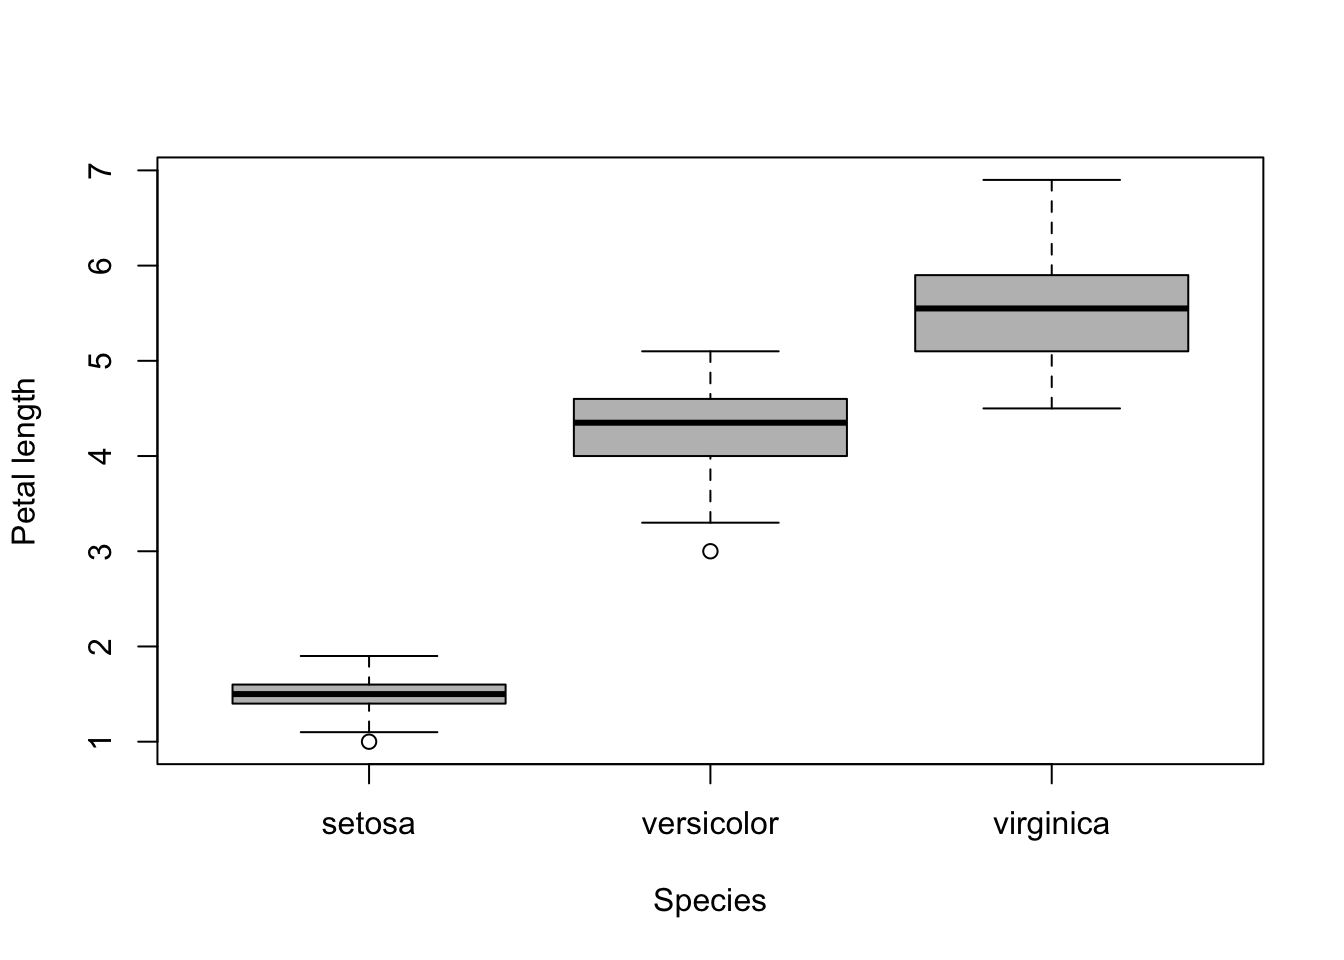
\includegraphics{005-figures_files/figure-latex/fig4-1-1.pdf}
\caption{\label{fig:fig4-1}\texttt{iris}数据集\texttt{Petal.Length\}\ \textasciitilde{}\ Species}的箱线图.}
\end{figure}

\hypertarget{sec5-2}{%
\section{\texorpdfstring{由\texttt{R}生成两个图形并置示例}{由R生成两个图形并置示例}}\label{sec5-2}}

在\texttt{R}的代码块选项中设置\texttt{out.width=\textquotesingle{}50\%\textquotesingle{}}, \texttt{fig.show=\textquotesingle{}hold\textquotesingle{}}就可获得二个图形的并置.



\begin{figure}
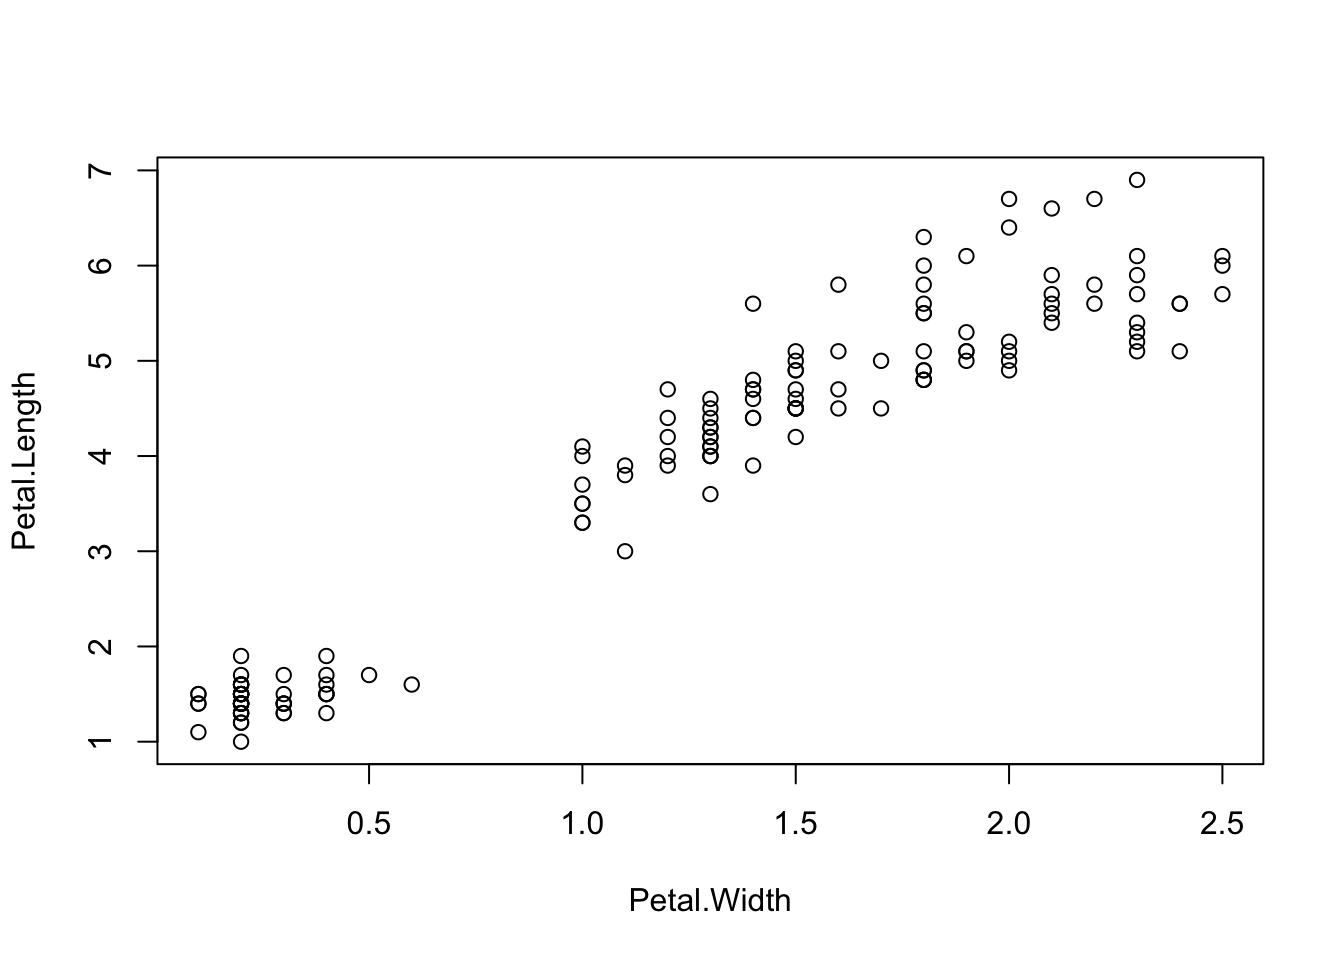
\includegraphics[width=0.5\linewidth]{005-figures_files/figure-latex/fig4-2-1} 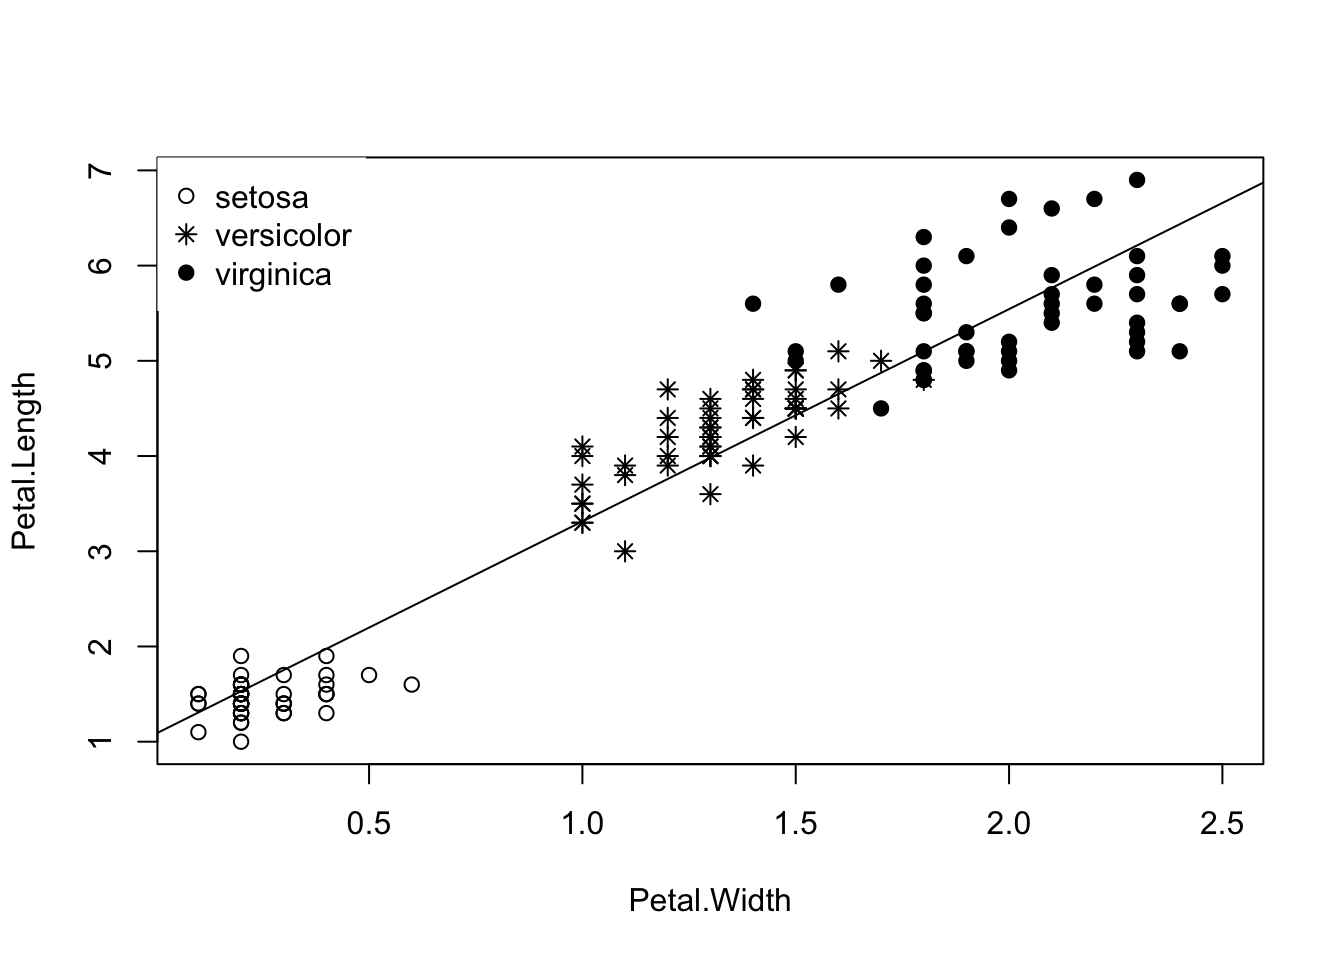
\includegraphics[width=0.5\linewidth]{005-figures_files/figure-latex/fig4-2-2} \caption{\texttt{iris}数据集\texttt{Petal.Length\}\ \textasciitilde{}\ Species} 的散点图. 右侧的图像中散点类型通过\texttt{Species}因子的水平给出,见图例. 直线为数据集拟合线性模型的结果.}\label{fig:fig4-2}
\end{figure}

\hypertarget{sec5-3}{%
\section{\texorpdfstring{由\texttt{R}生成两个图形堆叠示例}{由R生成两个图形堆叠示例}}\label{sec5-3}}

\indent

在\texttt{R}的代码块选项中设置\texttt{out.width=\textquotesingle{}90\%\textquotesingle{}}, \texttt{fig.show=\textquotesingle{}hold\textquotesingle{}}就可获得二个图形的并置.



\begin{figure}
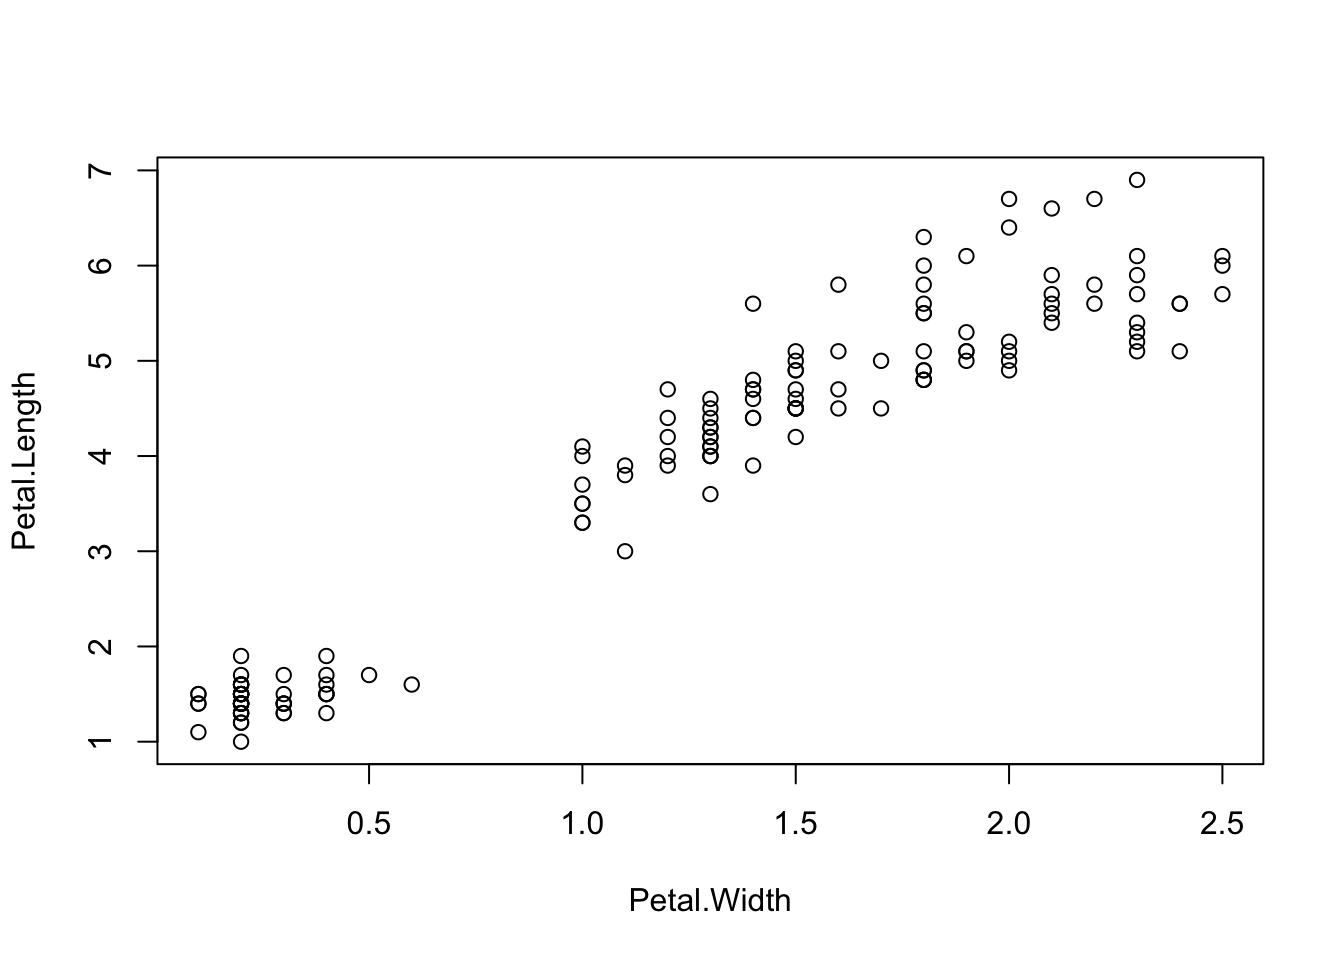
\includegraphics[width=0.9\linewidth]{005-figures_files/figure-latex/fig4-3-1} 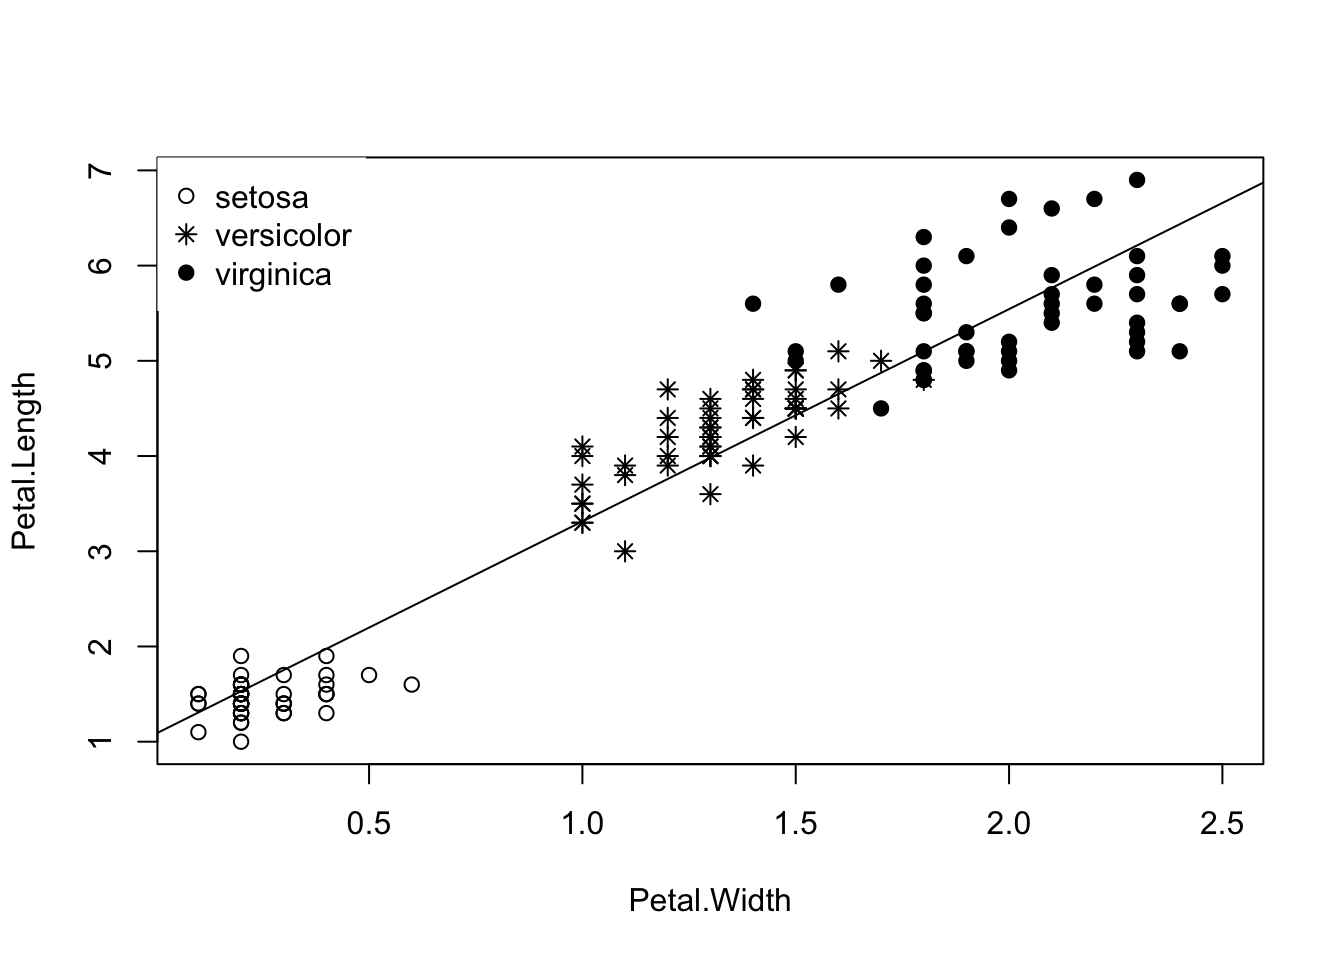
\includegraphics[width=0.9\linewidth]{005-figures_files/figure-latex/fig4-3-2} \caption{\texttt{iris}数据集\texttt{Petal.Length\}\ \textasciitilde{}\ Species} 的散点图. 下方的图像中散点类型通过\texttt{Species}因子的水平给出,见图例. 直线为数据集拟合线性模型的结果.}\label{fig:fig4-3}
\end{figure}

\hypertarget{sec5-4}{%
\section{静态图形示例}\label{sec5-4}}

\indent

在\texttt{Bookdwon}中插入本地图形可使用命令(示例为\texttt{R}logo)

\begin{Shaded}
\begin{Highlighting}[]
\NormalTok{knitr}\SpecialCharTok{::}\FunctionTok{include\_graphics}\NormalTok{(}\StringTok{"figures/Rlogo.png"}\NormalTok{)}
\end{Highlighting}
\end{Shaded}



\begin{figure}

{\centering 
\includegraphics[width=0.7\linewidth]{figures/Rlogo} 

}

\caption{R logo}\label{fig:fig4-4}
\end{figure}

\hypertarget{sec5-5}{%
\section{图形引用}\label{sec5-5}}

\indent

图形引用通过\texttt{R}代码块的标签引用, 并带前缀\texttt{fig:}, 例如

\begin{verbatim}
图\\ref{fig:fig4-2}和图\\ref{fig:fig4-3}为两个图的并置与堆叠. 
\end{verbatim}

输出为:

图\ref{fig:fig4-2}和图\ref{fig:fig4-3}为两个图的并置与堆叠.

\printbibliography[segment=\therefsegment, heading=subbibliography, title={参考文献}]

\hypertarget{tables}{%
\chapter{\texorpdfstring{\texttt{Bookdown}中的表格}{Bookdown中的表格}}\label{tables}}

\indent

这是第 \ref{tables} 章的内容, 讲述浮动对象图形的标签与引用. \autocite{xie2015,bookdown2016}

\hypertarget{sec6-1}{%
\section{表格示例1:由数据生成表格}\label{sec6-1}}

\begin{Shaded}
\begin{Highlighting}[]
\NormalTok{knitr}\SpecialCharTok{::}\FunctionTok{kable}\NormalTok{(}
  \FunctionTok{head}\NormalTok{(mtcars[, }\DecValTok{1}\SpecialCharTok{:}\DecValTok{5}\NormalTok{], }\DecValTok{10}\NormalTok{), }\AttributeTok{booktabs =} \ConstantTok{TRUE}\NormalTok{,}
  \AttributeTok{caption =} \StringTok{\textquotesingle{}mtcars数据的前5行.\textquotesingle{}}
\NormalTok{)}
\end{Highlighting}
\end{Shaded}

\begin{table}

\caption{\label{tab:tab3-1}mtcars数据的前5行.}
\centering
\begin{tabular}[t]{lrrrrr}
\toprule{}
  & mpg & cyl & disp & hp & drat\\
\midrule{}
Mazda RX4 & 21.0 & 6 & 160.0 & 110 & 3.90\\
Mazda RX4 Wag & 21.0 & 6 & 160.0 & 110 & 3.90\\
Datsun 710 & 22.8 & 4 & 108.0 & 93 & 3.85\\
Hornet 4 Drive & 21.4 & 6 & 258.0 & 110 & 3.08\\
Hornet Sportabout & 18.7 & 8 & 360.0 & 175 & 3.15\\
\addlinespace
Valiant & 18.1 & 6 & 225.0 & 105 & 2.76\\
Duster 360 & 14.3 & 8 & 360.0 & 245 & 3.21\\
Merc 240D & 24.4 & 4 & 146.7 & 62 & 3.69\\
Merc 230 & 22.8 & 4 & 140.8 & 95 & 3.92\\
Merc 280 & 19.2 & 6 & 167.6 & 123 & 3.92\\
\bottomrule{}
\end{tabular}
\end{table}

\hypertarget{sec6-2}{%
\section{表格示例2: 由数据框构造表格}\label{sec6-2}}

\indent



\begin{table}

\caption{\label{tab:tab3-2}遗传连接模型例子中观测到的频数 \(y_i\) 和频率 \(p(y_i|\pi)\),\(i=1, \dots ,4\),197个动物.}
\centering
\begin{tabular}[t]{lllll}
\toprule{}
Category & 1 & 2 & 3 & 4\\
\midrule{}
Frequency $y_i$ & 125 & 18 & 20 & 34\\
Probability $p(y_i\mid\pi)$ & $\frac{1}{2}+\frac{\pi}{4}$ & $\frac{1}{4}(1-\pi)$ & $\frac{1}{4}(1-\pi)$ & $\frac{1}{4}$\\
\bottomrule{}
\end{tabular}
\end{table}

注意:

\begin{enumerate}
\def\labelenumi{\arabic{enumi}.}
\tightlist
\item
  表格中\texttt{\%}用\texttt{\textbackslash{}\textbackslash{}\%}
\item
  表格中latex命令用\texttt{\textbackslash{}\textbackslash{}}代替\texttt{\textbackslash{}}
\end{enumerate}

\hypertarget{sec6-3}{%
\section{表格引用}\label{sec6-3}}

\indent

表格引用由代码块的标签(设为\texttt{label})引用实现, 并带前缀\texttt{tab:}, 由\texttt{\textbackslash{}@ref(tab:label)}实现. 例如

\begin{verbatim}
本章共出现二张表格,即表\\ref{tab:tab3-1}和表\\ref{tab:tab3-2}.
\end{verbatim}

输出为:

本章共出现二张表格,即表\ref{tab:tab3-1}和表\ref{tab:tab3-2}.

\textbf{注}: 表格中的caption(题图)由文本引用生成.

\printbibliography[segment=\therefsegment, heading=subbibliography, title={参考文献}]

\hypertarget{textref}{%
\chapter{\texorpdfstring{\texttt{Bookdown}中的文本参考}{Bookdown中的文本参考}}\label{textref}}

\indent

这是第\ref{textref}章的内容, 讲述文本的标签与引用. \autocite{xie2015,R-base}

\hypertarget{sec7-1}{%
\section{文本标签的设定与引用}\label{sec7-1}}

\indent

通过\texttt{(ref:label)}设定被引文本,其前后必须有空行与正文分开. 例如

\begin{verbatim}


被引用的文本: 我要被引用的**文本**.  
\end{verbatim}

输出为



被引用的文本: 我要被引用的\textbf{文本}.

\hypertarget{sec7-2}{%
\section{文本引用场景}\label{sec7-2}}

\indent

在\texttt{Bookdown}中文本引用主要用于图形与表格的题图(caption)上, 见第\ref{figures}章和第\ref{tables}章的例子.

\printbibliography[segment=\therefsegment, heading=subbibliography, title={参考文献}]

\hypertarget{bibs}{%
\chapter{\texorpdfstring{\texttt{Bookdown}中的文献排版}{Bookdown中的文献排版}}\label{bibs}}

\indent

这是第\ref{bibs}章的内容,讲解文献库的建立、文献格式与排版方法. \autocite{xie2015,R-base}

\hypertarget{sec8-1}{%
\section{文献库建立样例}\label{sec8-1}}

\indent

根据文献的类型,文献库的格式有14种类型,它们由\texttt{title},\texttt{author}, \texttt{journal},\texttt{address}等域构成. 最为常见的文献类型是论文(\texttt{article})和图书(\texttt{book}), 它们的格式如下

\begin{verbatim}
    @article{CitekeyArticle,
      author   = "P. J. Cohen",
      title    = "The independence of the continuum hypothesis",
      journal  = "Proceedings of the National Academy of Sciences",
      year     = 1963,
      volume   = "50",
      number   = "6",
      pages    = "1143--1148",
    }
\end{verbatim}

\begin{verbatim}
    @book{CitekeyBook,
      author    = "Leonard Susskind and George Hrabovsky",
      title     = "Classical mechanics: the theoretical minimum",
      publisher = "Penguin Random House",
      address   = "New York, NY",
      year      = 2014
    }
\end{verbatim}

其余类型参见网页:\href{https://www.bibtex.com/e/entry-types/}{The 14 BibTeX entry types}。
文献库通过\texttt{BiBTeX}或\texttt{BiBer}的运行生成文献目录(bibliography).

\hypertarget{sec8-2}{%
\section{文献风格}\label{sec8-2}}

\indent

不同的期刊、书集对文献目录中参考文献的呈现方式有不同的要求,\texttt{BiBTeX}是通过风格(style)文件来控制(配合宏包\texttt{natbib}使用), \texttt{BiBer}是通过选项来控制(配合\texttt{biblatex}使用).

文献呈现的风格分为作者-日期格式(author-date style)和数字格式(numeric)。作者-日期格式共有141个式样,其中最为常用的式样有2个,即\texttt{alpha}和\texttt{apalike}。 数据格式共88个式样,其中有8类是标准式样,也是最常用的式样,即\texttt{abbrv}, \texttt{acm},\texttt{ieeetr},\texttt{plain},\texttt{siam}, 和\texttt{unsrt}。这些式样的具体形式与介绍见\href{https://www.bibtex.com/styles/}{}

中文的文献排版根据国标GB/T77114-2015的规范,对文献的类型要求提供文献的标识代码,共有18个,例如图书用\texttt{M}标识,期刊论文用\texttt{J}标识。

\hypertarget{sec8-3}{%
\section{中文文献风格的设置}\label{sec8-3}}

\indent

基于\texttt{BiBTeX}, 中文文献通过宏包\texttt{gbt7714}实现\footnote{详见 \url{https://github.com/87ouo/gbt7714-bibtex-style} 说明},兼容宏包\texttt{natbib},在\(\LaTeX\)中使用方法如下:

\begin{enumerate}
\def\labelenumi{\arabic{enumi}.}
\item
  在导言区调用宏包 \texttt{gbt7714};
\item
  在正文中 \texttt{\textbackslash{}cite\{\}}等引用文献;
\item
  使用 \texttt{\textbackslash{}bibliographystyle\{\}} 选择参考文献表的样式;
\item
  使用 \texttt{\textbackslash{}bibliography\{\}} 命令生成参考文献表;
\item
  编译生成带文献的pdf文件,基于\texttt{xelatex}引擎的编译方式如下(\texttt{foo.tex}为文件名)
\end{enumerate}

\begin{verbatim}
    xelatex foo.tex
    bibtex foo
    xelatex foo.tex
    xelatex foo.tex
\end{verbatim}

基于\texttt{BiBer}, 中文文献通过宏包\texttt{biblatex-gb7714-2015} 实现\footnote{详见 \url{https://github.com/hushidong/biblatex-gb7714-2015}},兼容宏包\texttt{biblatex}。本质上\texttt{biblatex-gb7714-2015} 是个式样宏包,依附于宏包\texttt{biblatex}, 通过式样选项使用. 在\(\LaTeX\)中使用方法如下:

\begin{enumerate}
\def\labelenumi{\arabic{enumi}.}
\item
  在导言区调用宏包 \texttt{biblatex}, 并设定文献样本和, 例如;

  \begin{itemize}
  \tightlist
  \item
    使用顺序编码制:
  \end{itemize}

\begin{verbatim}
\usepackage[backend=biber,style=gb7714-2015]{biblatex}
\end{verbatim}

  \begin{itemize}
  \tightlist
  \item
    使用著者-出版年制\footnote{尽管后端(\texttt{backend})可以使用\texttt{bibtex}, 但不建议使用.}:
  \end{itemize}

\begin{verbatim}
 \usepackage[backend=biber,style=gb7714-2015ay]{biblatex}
\end{verbatim}
\item
  在\texttt{\textbackslash{}begin\{document\}}加载参考文献库,命令为\texttt{\textbackslash{}addbibresource\{\}}
\item
  在正文中 \texttt{\textbackslash{}cite\{\}} 等引用文献;
\item
  在需要出现文献目录的地方使用 \texttt{\textbackslash{}printbibliography},可通过\texttt{title}, \texttt{heading}, \texttt{segment}选项对输出进行控制;
\item
  编译生成带文献的\texttt{pdf}文件,基于\texttt{xelatex}引擎的编译方式如下(\texttt{foo.tex}为文件名)
\end{enumerate}

\begin{verbatim}
    xelatex foo.tex
    biber foo
    xelatex foo.tex
    xelatex foo.tex
\end{verbatim}

\hypertarget{sec8-4}{%
\section{文献库的建立工具}\label{sec8-4}}

\begin{itemize}
\item
  Zotero
\item
  JabRef
\end{itemize}

\printbibliography[segment=\therefsegment, heading=subbibliography, title={参考文献}]

\cleardoublepage

\hypertarget{appendix-ux9644ux5f55}{%
\appendix \addcontentsline{toc}{chapter}{\appendixname}}


\hypertarget{mjx}{%
\chapter{\texorpdfstring{\texttt{Mathjax}的离线安装与使用}{Mathjax的离线安装与使用}}\label{mjx}}

\indent

附录\ref{mjx}介绍了网页显示数学公式的插件mathjax,本地化安装,使用方法等. \autocite{xie2015,R-base}

\hypertarget{sec9-1}{%
\section{mathjax 说明}\label{sec9-1}}

\begin{itemize}
\item
  \href{https://www.mathjax.org/}{MathJax}是一款相当强悍的在网页显示数学公式的插件。基于\texttt{Mathjax}, 通过\(\LaTeX\)的命令输出精美的数学公式. 加载Mathjax后\footnote{需要运程或本地支持},就可通过一对美元符号\texttt{\$}(或左\texttt{\textbackslash{}(}右 \texttt{\textbackslash{})})输入行内公式,通过一对双美元符号\texttt{\$\$}(或左\texttt{\textbackslash{}{[}}右\texttt{\textbackslash{}{]}})输入行间公式,例如

\begin{verbatim}
$$
J\alpha(x) = \sum{m=0}^\infty \frac{(-1)^m}{m! \Gamma (m + \alpha + 1)} {\left({ \frac{x}{2} }\right)}^{2m + \alpha}
$$
\end{verbatim}

  显示出下面的数学公式
  \[
  J\alpha(x) = \sum{m=0}^\infty \frac{(-1)^m}{m! \Gamma (m + \alpha + 1)} {\left({ \frac{x}{2} }\right)}^{2m + \alpha}
  \]
\item
  可以使用\(\LaTeX\)自带的复杂的数学环境,如排版多行公式的\texttt{align}, \texttt{split}和数学字体命令,如\texttt{\textbackslash{}mathscr}
\end{itemize}

\begin{verbatim}
\begin{align}
3x-1 &= \mathbb{A} \\
  3x &= \mathbf{B} \\
   x &= \mathscr{C}
\end{align}
\end{verbatim}

输出为
\begin{align}
3x-1 &= \mathbb{A} \\
  3x &= \mathbf{B} \\
   x &= \mathscr{C}
\end{align}

\hypertarget{sec9-2}{%
\section{\texorpdfstring{调用远程服务器上的\texttt{mathjax}}{调用远程服务器上的mathjax}}\label{sec9-2}}

\indent

一般情况下,只需要使用远程加载\texttt{Mathjax}的\texttt{js}库就行了,例如在需要渲染数学公式的网页上增加\texttt{html}命令

\begin{verbatim}
</script>
<script type="text/javascript" async
  src="https://cdn.mathjax.org/mathjax/latest/MathJax.js?config=TeX-MML-AM_CHTML">
</script>
\end{verbatim}

\hypertarget{sec9-3}{%
\section{\texorpdfstring{\texttt{mathjax}本地服务器的安装与使用}{mathjax本地服务器的安装与使用}}\label{sec9-3}}

\indent

我们以\texttt{Macbook}的\texttt{Apache}服务器为例说明步骤\footnote{Windows 10下的本地服务器的启动可参考(\url{https://www.jianshu.com/p/d86c77942181})}

\begin{enumerate}
\def\labelenumi{\arabic{enumi}.}
\tightlist
\item
  服务器的启动
\end{enumerate}

在终端(terminal)下输入命令

\begin{verbatim}
sudo apachectl start
\end{verbatim}

\begin{enumerate}
\def\labelenumi{\arabic{enumi}.}
\setcounter{enumi}{1}
\tightlist
\item
  检查服务是否启动成功
\end{enumerate}

在浏览器中输入网址

\begin{verbatim}
http://127.0.0.1/ 
\end{verbatim}

如果显示\texttt{It\ Works!}就表示服务器已经成功启动。请记住:服务器上文件在本地的位置为

\begin{verbatim}
/Library/WebServer/Documents
\end{verbatim}

\begin{enumerate}
\def\labelenumi{\arabic{enumi}.}
\setcounter{enumi}{2}
\tightlist
\item
  关闭服务器(不用时)
\end{enumerate}

在终端(terminal)下输入命令

\begin{verbatim}
sudo apachectl stop
\end{verbatim}

\begin{enumerate}
\def\labelenumi{\arabic{enumi}.}
\setcounter{enumi}{3}
\item
  将\texttt{Mathjax2.6}或\texttt{Mathjax2.7}下载并解压(安装)到\texttt{/Library/WebServer/Documents}下\footnote{不要用最新的3.1版本}, 目录名为\texttt{Mathjax}
\item
  启动本地\texttt{Mathjax}
\end{enumerate}

在运行\texttt{Bookdown}(或其他\texttt{rmarkdown}文件)时,须加载下面的\texttt{html}命令,在\texttt{Bookdown}中放在文件\texttt{mathjax\_header.html}中,并由\texttt{\_output.yml}加载进来.

\begin{verbatim}
</script>
<script type="text/javascript"
   src="http://127.0.0.1/MathJax/MathJax.js">
</script>
\end{verbatim}

\printbibliography[segment=\therefsegment, heading=subbibliography, title={参考文献}]

\hypertarget{biber}{%
\chapter{\texorpdfstring{基于\texttt{biblatex}生成参考文献}{基于biblatex生成参考文献}}\label{biber}}

附录\ref{biber}介绍了 文献库扩展包\texttt{biblatex}的使用,及其与\texttt{natbib}的比较. \autocite{xie2015,R-base}

\hypertarget{sec10-1}{%
\section{bibtex 与 biber, natbib 与 biblatex 比较}\label{sec10-1}}

\hypertarget{ux6982ux8ff0}{%
\subsection{概述}\label{ux6982ux8ff0}}

\begin{itemize}
\item
  \texttt{bibtex} 与 \texttt{biber} 是处理参考文献信息二个外部程序(backend), 它们起
  到将\(\LaTeX\) 文档与 \texttt{bib} 文档交互的作用;
\item
  \texttt{natbib} 与 \texttt{biblatex} 是二个处理参考文献(bibliography) 和引用(citation)的\(\TeX\) 宏包; \texttt{natbib} 仅通过\texttt{bibtex} 起作用,而\texttt{biblatex} 可通过
  \texttt{biber} 起作用;
\end{itemize}

\hypertarget{natbib-ux7684ux4f18ux70b9}{%
\subsection{\texorpdfstring{\texttt{natbib} 的优点}{natbib 的优点}}\label{natbib-ux7684ux4f18ux70b9}}

\begin{itemize}
\item
  natbib 的优点:

  \begin{itemize}
  \tightlist
  \item
    有大量与期刊/出版商对应的风格文件(.sty);
  \end{itemize}
\item
  natbib 的缺点:

  \begin{itemize}
  \item
    修改风格文件较为困难;
  \item
    其设计的局限性:主要为自然科学类期刊的\texttt{Author-Year} 及数字引
    用方式设计.
  \end{itemize}
\end{itemize}

\hypertarget{biblatex-ux7684ux4f18ux7f3aux70b9}{%
\subsection{biblatex 的优缺点}\label{biblatex-ux7684ux4f18ux7f3aux70b9}}

\begin{itemize}
\item
  \texttt{biblatex} 被认为是\(\LaTeX\) 中处理参考文献(bibliography) 的很有前途的宏包,功能强大,提供了很多可定制选项。
\item
  \texttt{biblatex} 的优点

  \begin{itemize}
  \tightlist
  \item
    提供\texttt{natbib} 的 \texttt{Author-year} 和数字引用方式,因此可视为natbib
    的扩展;
  \item
    通过\(\LaTeX\) 的宏控制文献的风格,方便修改;
  \item
    提供许多人性化的引用风格(例如\texttt{author-title});
  \item
    提供人性化的文献数据库域名(字段);
  \item
    直接支持多文献库与文献分类;
  \item
    提供大量标准与拓展的\texttt{biblatex} 风格(见使用手册);
  \item
    文献可按主题分割为部分;
  \end{itemize}
\end{itemize}

\hypertarget{sec10-2}{%
\section{\texorpdfstring{biblatex 的在\(\TeX\)中的使用样例}{biblatex 的在\textbackslash TeX中的使用样例}}\label{sec10-2}}

\begin{enumerate}
\def\labelenumi{\arabic{enumi}.}
\tightlist
\item
  使用
\end{enumerate}

\begin{verbatim}
  \usepackage[style=authoryear,backend=biber]{biblatex}
\end{verbatim}

(代替\texttt{\textbackslash{}usepackage{[}authoryear{]}\{natbib\}});

\begin{enumerate}
\def\labelenumi{\arabic{enumi}.}
\setcounter{enumi}{1}
\tightlist
\item
  加载一个或多个 \texttt{bib} 文献库文件:
\end{enumerate}

\begin{verbatim}
  \addbibresource{file1.bib}    
  \addbibresource{file2.bib}
\end{verbatim}

\begin{enumerate}
\def\labelenumi{\arabic{enumi}.}
\setcounter{enumi}{2}
\tightlist
\item
  要出现文献的地方输入
\end{enumerate}

\begin{verbatim}
  \printbibliography
\end{verbatim}

\begin{enumerate}
\def\labelenumi{\arabic{enumi}.}
\setcounter{enumi}{3}
\item
  引用: 使用\texttt{\textbackslash{}textcite} 代替\texttt{\textbackslash{}citet}; 使用\texttt{\textbackslash{}parencite} 代替\texttt{\textbackslash{}citep}
\item
  编译方式
\end{enumerate}

\begin{verbatim}
XELATEX(或LATEX, pdfLATEX)
biber(代替bibtex)
XELATEX(或LATEX, pdfLATEX)
XELATEX(或LATEX, pdfLATEX)
\end{verbatim}

\hypertarget{sec10-3}{%
\section{\texorpdfstring{\texttt{biblatex}在\texttt{bookdown}中的使用}{biblatex在bookdown中的使用}}\label{sec10-3}}

\begin{enumerate}
\def\labelenumi{\arabic{enumi}.}
\item
  在\texttt{index.Rmd}文件的\texttt{yml}部分增加选项

\begin{verbatim}
biblatexoptions: [refsegment=chapter]
biblio-style: gb7714-2015ay
\end{verbatim}

  注意\texttt{{[}{]}}内可增加其他\texttt{biblatex}选项(参考\texttt{biblatex}使用手册)
\item
  在需要出现文献的地方(如每一章后)加

\begin{verbatim}
\printbibliography[segment=\therefsegment, heading=subbibliography, title={参考文献}]
\end{verbatim}
\item
  在\texttt{\_output.yml}文件的\texttt{bookdown::pdf\_book:}增加选项(前面空二格)

\begin{verbatim}
 citation_package: biblatex
\end{verbatim}

  注:若要\texttt{bibtex}驱动文献的排版,只需要在这一步改为\texttt{citation\_package:\ natbib}
\item
  如上所述,LaTeX 要生成最终的 PDF 文档,如果含有交叉引用(图形、表格、公式、章节、文献等)、BibTeX/biber、术语表等等,通常需要多次编译才行。而使用 Latexmk 则只需运行一次,它会自动帮你做好其它所有事情。尽管在你已经安装的 LaTeX 发行版本已经包含了 Latexmk,但我们需要运行它。使用\texttt{XeLaTeX}的编译格式为
\end{enumerate}

\begin{verbatim}
latexmk -pvc -xelatex file.tex
\end{verbatim}

其中选项\texttt{pvc}表示检查输入文件的更改并预览结果。在Rstudio中你只需要添加下面的代码块。

\begin{Shaded}
\begin{Highlighting}[]
\FunctionTok{Sys.setenv}\NormalTok{(}\AttributeTok{RSTUDIO\_PDFLATEX =} \StringTok{"latexmk"}\NormalTok{)}
\end{Highlighting}
\end{Shaded}

\printbibliography[segment=\therefsegment, heading=subbibliography, title={参考文献}]

\printbibliography

\backmatter

\printindex

\end{document}
